\documentclass{amsart}
\usepackage{graphicx}
\graphicspath{{./}}
\usepackage{hyperref}
\usepackage{csvsimple}
\usepackage{longtable}
\usepackage{epigraph}
\title{Graphical Assessment of Ethnicity-Independence of Human Moral Nature}
\author{Zulfikar Moinuddin Ahmed}
\date{\today}
\begin{document}
\maketitle

\section{Introduction}

The universal human moral nature that is ethnicity-independent is my discovery, and one of my greatest discoveries.  It is such a profound discovery that I feel that it is Fate that propels me forward to end all ethnic strife on Earth, and that this, among others, was the purpose of my birth on Earth.  

In a previous note, I conducted a paired t-test for ethnicity pairs and found strong evidence that as vectors the 10-dimensional probability vectors are statistically indistinguishable.

Here I provide you with the visual display of the probability densities that gives us compelling evidence that these distributions are minor perturbations of each other and are not significantly different.


\section{Line Graphs}

\includegraphics[scale=0.7]{q177.jpeg}

\includegraphics[scale=0.7]{q178.jpeg}


\includegraphics[scale=0.7]{q179.jpeg}

\includegraphics[scale=0.7]{q180.jpeg}

\includegraphics[scale=0.7]{q181.jpeg}

\includegraphics[scale=0.7]{q182.jpeg}

\includegraphics[scale=0.7]{q183.jpeg}

\includegraphics[scale=0.7]{q184.jpeg}

\includegraphics[scale=0.7]{q185.jpeg}

\includegraphics[scale=0.7]{q186.jpeg}

\includegraphics[scale=0.7]{q187.jpeg}

\includegraphics[scale=0.7]{q188.jpeg}

\includegraphics[scale=0.7]{q189.jpeg}

\includegraphics[scale=0.7]{q190.jpeg}

\includegraphics[scale=0.7]{q191.jpeg}

\includegraphics[scale=0.7]{q192.jpeg}

\includegraphics[scale=0.7]{q193.jpeg}

\includegraphics[scale=0.7]{q194.jpeg}

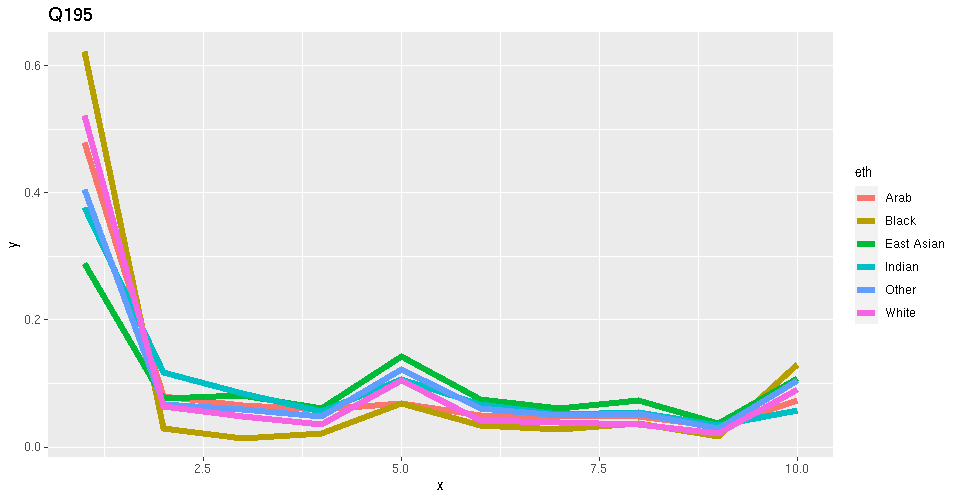
\includegraphics[scale=0.7]{q195.jpeg}

\section{Precise Variation Explained By Ethnicity}

We consider a measure that is like $R^2$ now to tabulate the effect of ethnicity on moral value distribution.  We compute this as residual sum of squares divided by total sum of squares wih respect to the mean mean curve over ethnicities.

% latex table generated in R 4.0.3 by xtable 1.8-4 package
% Sat May  8 00:26:41 2021
\begin{table}[ht]
\centering
\begin{tabular}{rlr}
  \hline
 & eth & explained \\ 
  \hline
1 & Arab & 4.82 \\ 
  2 & Black & 3.75 \\ 
  3 & East Asian & 4.85 \\ 
  4 & Indian & 7.73 \\ 
  5 & Other & 1.89 \\ 
  6 & White & 6.07 \\ 
   \hline
\end{tabular}
\end{table}

We get values roughly between 2-8\%.  This is reasonable and fairly small, and quite mysterious.  Across the world, we {\em share} almost identical moral value preferences with ethnic variation in this range 2-8\%.  
\end{document}